%CS 109 Problem Set Xiaoqi Zhou


\documentclass{article}
	% basic article document class
	% use percent signs to make comments to yourself -- they will not show up.

\usepackage{amsmath}
\usepackage{amssymb}
	% packages that allow mathematical formatting

\usepackage{graphicx}
\usepackage{float}
	% package that allows you to include graphics

\usepackage[top=1in, bottom=1in, left=1in, right=1in]{geometry}

\frenchspacing
	% one space after periods

\usepackage{fancyhdr}
	% allows custom headers

\pagestyle{fancy}

\lhead{CS 109, Stanford University \\ Problem Set \#5} 
\rhead{Xiaoqi Zhou (xqzhou@stanford.edu) \\ 06237147}
\usepackage{color}
\usepackage{courier}
\usepackage{relsize}
\cfoot{\thepage}
\renewcommand{\footrulewidth}{0.4pt} 
	%footer
\newcommand{\myansw}{\textbf{Answer:}\\}
\newcommand{\mysolu}{\textbf{Solution:}\\}
\begin{document}
\thispagestyle{fancy} %shows header/footer

\begin{enumerate}
	\item
	%1
	\begin{enumerate}
		\item
		\myansw
		The after trial distribution is:\\
		\colorbox{yellow}{${f(x) = Beta(2+7, 2+2)  = Beta(9,4)}$}\\
		\item
		\myansw
		${F_{Beta}(0.5) = 0.073}$\\
		\colorbox{yellow}{${P(\text{drug having effect} \geq 0.5) = 1 - F_{Beta}(0.5) = 0.927}$}\\
		
	
		
	\end{enumerate}
	\item
	\begin{enumerate}
		\item
		\myansw
		${P(35 \leq X \leq 40) = 0.00022}$\\
		${P(40 \leq X \leq 45) = 0.04192}$\\
		${P(60 \leq X \leq 65) = 0.00022}$\\
		
		\begin{figure}[H]
			\centering
			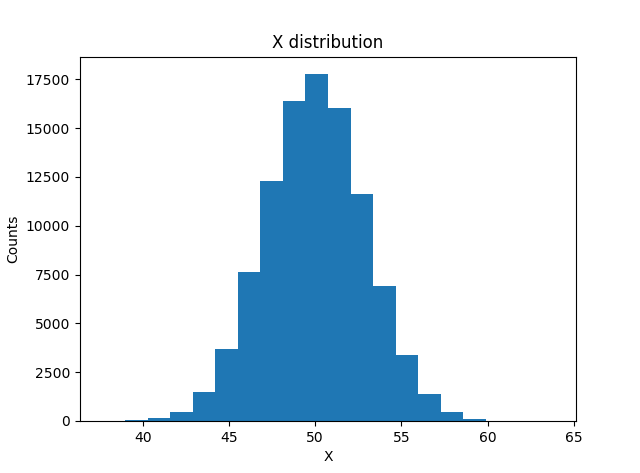
\includegraphics[width=0.8\textwidth]{pset_5_2_a.png}
		\end{figure}
		\item
		\mysolu
		From the simulation results, we can find\\
		${E[X] = 50.00}$\\
		${Var(X) = 8.336}$\\
		Then we can use normal distribution to represent the distribution.\\
		\myansw
		\colorbox{yellow}{${X \sim N(50.00, 8.336)}$}\\
		\colorbox{yellow}{${f(x) = \frac{1}{\sqrt{2\pi8.336}}e^{-(x-50)^2/(2\times 8.336)}}$}\\
		\item
		\mysolu
		${P\{40 \leq X \leq 45\}= F(45) - F(40) =\Phi(\frac{(45 -50)}{\sqrt{8.336}}) -  \Phi(\frac{(40 -50)}{\sqrt{8.336}})}$\\
		\colorbox{yellow}{text${P\{40 \leq X \leq 45\}= \Phi(\frac{10}{2.89}) -  \Phi(\frac{5}{2.89}) = 0.9997 - 0.9582 = 0.0415}$}\\
		
		
		
	\end{enumerate}
	\item
	\begin{enumerate}
	\item
		\myansw
		The expected amount of money that each person gives is\\
		\colorbox{yellow}{${E[X] = 5.95}$}\\
		\item
		\myansw
		\colorbox{yellow}{${Var(X) = E[X^2]-(E[X])^2 = 23.19}$}\\
		\item
		\mysolu
		${E[n\overline{X}]= nE[X]= 5.95 \times 50 =279.5}$\\
		${Var(n\overline{X}) = nVar(X)=1159.5}$\\
		\myansw
		\colorbox{yellow}{${\sum\limits_{i = 1}^{50}X_i \sim N(279.5, 1159.5)}$}\\		
		\item
		\myansw
		${Y = \sum\limits_{i = 1}^{50}X_i}$\\
		\colorbox{yellow}{${P\{Y \geq 350\} = 1 - P\{Y < 350\} = 1 - \Phi(\frac{350 - 279.5}{\sqrt{1159.5}}) = 1 - 0.9808  = 0.02}$}
		

	\end{enumerate}
	\item
	\mysolu 
	${Cov(X,Y) = Cov(X,X^2) = E[X^3] - E[X]E[X^2]}$\\
	$E[X^3] = \frac{1}{6}\sum\limits_{i = 1}^{6}i^3 = 73.5$\\
	$E[X^2] = \frac{1}{6}\sum\limits_{i = 1}^{6}i^2 = 15.17$\\
	$E[X] =\frac{1}{6}\sum\limits_{i = 1}^{6}i = 3.5 $\\
	\myansw
	\colorbox{yellow}{${Cov(X,Y) = 20.65}$}\\
	
	\item 
	\myansw
	\colorbox{yellow}{${2X + Y \sim N(2+1, 2\times 2 + 2)}$}\\
	\colorbox{yellow}{${2X + Y \sim N(3, 6)}$}\\
	\item
	\begin{enumerate}
		\item 
		\myansw
		\colorbox{yellow}{$f(x) = \frac{1}{4\sqrt{2\pi}}e^{-(x-98)^2/32}$}\\
		\item
		\myansw
		Let Y be the measured distance\\
		\colorbox{yellow}{$f(y = 100|x = t) = \frac{1}{2\sqrt{2\pi}}e^{-(100-t)^2/8}$}\\
		\item
		\mysolu
		$f(x, y = 100) =f(y = 100|x )f(x)=\frac{1}{2\sqrt{2\pi}}e^{-(100-x)^2/8}\times \frac{1}{4\sqrt{2\pi}}e^{-(x-98)^2/32} $\\
		$\mathlarger{f(x | y = 100) = \frac{f(y = 100, x)}{f(y = 100)} = \frac{f(y = 100, x)}{\mathlarger{\int_{-\infty}^{+\infty}f(y = 100)dx}}}$\\
	\end{enumerate}
	
	
	
	
	
\end{enumerate}


\newpage



\end{document}